\documentclass[10pt]{article}
\usepackage[margin=1in]{geometry}
\usepackage{amsmath,amssymb,booktabs,graphicx,multirow,hyperref,xcolor,placeins,float}
\usepackage[numbers,super,sort&compress]{natbib}
\hypersetup{colorlinks=true,citecolor=blue,urlcolor=blue,linkcolor=blue,hypertexnames=false}
\title{Prioritizing gene and combination assays in the Norman--Weissman K562 Perturb-seq screen}
\author{Jinluo research team\\
Affiliation and corresponding-author details: to be supplied by the submitting authors}
\date{}
\begin{document}
\maketitle

\begin{abstract}
In the Norman--Weissman K562 Perturb-seq screen, a screening scientist may need to choose which gene or gene-combination perturbations to assay first under a fixed throughput budget. We test an auditable contract for that decision: 512 identity-gene indicators, 256 Reactome scores, 102 component indicators and known gemgroup metadata predict a 512-gene control-relative response. A multi-output ridge is trained on identity-by-gemgroup means and compared with aggregation-matched controls under locked identity splits. Across five confirmation splits, the batch-conditioned model has lower RMSE and higher Pearson and Spearman point estimates in every split: mean RMSE $0.3234$ versus $0.3240$, Pearson $0.1515$ versus $0.1385$, and Spearman $0.1080$ versus $0.0919$. Fixed-rank identity-cluster sensitivity intervals are descriptive because the splits are not biological replicates. In a locked retrospective prioritization evaluation, the model ranked 27 untouched combinations after validation-only penalty selection; mean top-$k$ overlap was 0.60, 0.76 and 0.89 at $k=5$, $10$ and $20$, versus random $k/27$ nulls of 0.185, 0.370 and 0.741. Locked pathway Spearman was 0.846, but top-$5$ cross-seed Jaccard was 0.056. The evidence supports an observed-gemgroup within-Norman operating regime and a bounded assay-shortlist aid, not causal pathway activation, unseen-batch transfer, clinical benefit or universal superiority.
\end{abstract}

\section{Introduction}
The practical value of a perturbation predictor is ultimately measured by the experiments it helps prioritize. In a disease-mechanism or target-discovery program, a screen can contain more plausible interventions than can be followed up at the bench. A model can therefore be useful as a retrospective decision aid if its highest-ranked gene or combination perturbations are enriched for large, reproducible transcriptional responses and if that enrichment is visible at a pathway level. In practice, a screening scientist or translational biologist could use the ranked list to decide which combinations to synthesize or assay first under a fixed throughput budget; the output changes assay order rather than treatment. This interpretation concerns selection of candidates for experimental testing; it does not imply clinical efficacy, therapeutic benefit or a causal mechanism. The Norman--Weissman K562 screen is a controlled proof-of-principle for this decision problem rather than a disease cohort, so any target-priority statement here is limited to the measured perturbation system.

Perturb-seq and related single-cell CRISPR assays connect a genetic intervention to a transcriptomic phenotype in the same cell. The experimental design is powerful because pooled guides provide many interventions while single-cell readout retains heterogeneity, but the design also introduces several sources of variation. Guide capture, library depth, cell quality, sequencing date and reagent handling can shift the measured expression distribution even when the perturbation identity is unchanged. These technical effects are part of the observed response and can be especially consequential when a predictor is evaluated at the cell level rather than on a single pseudobulk profile. The first Perturb-seq studies demonstrated the scale of this setting, with pooled genetic screens revealing molecular circuits and unfolded-protein-response programs across thousands of cells \citep{dixit2016,adamson2016}. Subsequent screens extended the design to combinatorial interventions and genome-scale genotype--phenotype maps \citep{datlinger2017,gasperini2019,mcfalinefigueroa2019,schraivogel2020,pmid32231336,pmid35688146,replogle2022}.

Prediction of perturbation responses has therefore become a useful complement to experimental screening. scGen transfers a state difference in a latent space, while CPA adds compositional and dose-aware factors \citep{lotfollahi2019,lotfollahi2020}. Graph and message-passing models such as GEARS encode perturbations and response genes jointly and target unseen combinations \citep{roohani2023}. Other systems use variational models, optimal transport, transformers and pretrained single-cell representations \citep{lopez2018,lotfollahi2022,geneformer2023,pmid35510185,pmid37154091,pmid34139164,pmid36608654,pmid36755098,pmid38844628,pmid40759747,scbert2022,qi2024}. Pathway-level neural decoders, including the in-house Pathway-NEAT-style implementation evaluated here, and neural additive model (NAM)-style decompositions provide a route from gene-level predictions to interpretable pathway hypotheses; they still require an information contract that excludes endpoint leakage. These methods have different estimands and different assumptions about the information available at inference. A predictor that receives the perturbed cell's endpoint expression answers a state reconstruction question; a predictor that receives only intervention identity and known assay-batch metadata answers a batch-aware intervention-to-response question. Mixing these contracts makes numerical comparisons hard to interpret. Large-scale guide-capture screens, perturbation atlases and cell-state references further show that guide assignment, replicate structure and annotation quality can alter the apparent response distribution \citep{pmid31422865,pmid33243861,pmid38772369,pmid37053306}. We therefore treat the identity and batch metadata as part of the estimand and record their provenance before fitting.

Technical covariates are often handled implicitly during preprocessing or integration. Normalization and batch-correction methods can remove reproducible assay variation or make the estimand dependent on a fitted latent representation \citep{wolf2018,stuart2019,haghverdi2018,korsunsky2019,gayoso2021,mimitou2019,stoeckius2017,cao2018,pmid34017005,pmid34584091}. A transparent alternative is to expose a known assay-batch label as an input and test whether conditioning on it improves predictions for cells carrying perturbation identities that were never used for fitting. The test is deliberately conservative: the same perturbation features, output genes, frozen control-relative target and identity split are used for every estimator. The factorial control separates identity-wide versus identity-by-gemgroup aggregation from the presence of the batch block.

Biological prior features can make this contract more informative without turning a predictor into a causal model. Reactome provides a curated hierarchy of molecular events and gene memberships \citep{reactome2020,pmid29377902,pmid29378288}. A perturbation identity can be represented by its indicator genes, the corresponding pathway scores and indicators for the observed component genes in a combination. These features describe what was perturbed before the endpoint is measured. They are not a claim that a Reactome annotation was activated in the cell. The distinction is essential: a coefficient or ablation result demonstrates predictive utility under a particular screen design, while causal activation requires intervention, temporal and mechanistic evidence that is absent from this analysis.

We focus on the Norman--Weissman screen because it contains many single and paired identities and a large number of measured cells in one cell line \citep{pmid31395745}. The primary task is to predict a 512-gene control-relative response for every held-out cell. The output is defined relative to observed control cells from the same archive so that a model is evaluated on intervention-specific change rather than on a shared housekeeping abundance. The identity split is performed before any model selection. Consequently, cells carrying an identity in confirmation are never used to estimate an identity mean, choose a penalty or determine a feature panel. This design addresses a common leakage route in which a random cell split places the same guide identity in both training and test.

Our contribution is a complete and bounded prediction system. First, we specify an input contract that contains 512 identity-gene indicators, 256 Reactome scores, 102 component indicators and known assay-batch metadata; endpoint expression, library size, guide count and response-derived statistics are excluded. Second, we fit a multi-output ridge model to identity-by-gemgroup means while freezing an independent control reference before any identity split. Third, we compare identity-wide and identity-by-gemgroup aggregation with and without the batch block using five validation-selected and locked confirmation splits, identity-cluster intervals for all three metrics, response-stratified analyses and feature-block ablations. The resulting claim is limited to the measured cell-level Norman operating regime. Cross-archive and cross-cell-line transfer are not inferred, and the model is not presented as a causal pathway simulator.

\section{Results}
\subsection{A fixed cell-level prediction contract}
The analysis began with the public Norman--Weissman h5ad release used for all primary results. The raw object contains 111,445 cells and 33,694 gene features. We retained 59,879 cells using the deterministic label-stratified sampling procedure defined before model fitting; 6,382 of these cells are controls. The sampled cells retain their source row indices, perturbation labels and gemgroup values, which allows the feature and response arrays to be audited against the original observation table. Eight gemgroups are represented in the sampled object. The control label is defined by the deterministic parser used during preprocessing: missing-like labels and explicit control or negative tokens map to the single CONTROL identity, while other labels preserve their perturbation components. In the filtered object the raw control category is recorded as ``control'' and contains 11,855 cells before sampling; no additional hidden control category was introduced during analysis.

Each sampled cell is associated with one perturbation identity. A single perturbation contributes one component token and a combination contributes one token for every retained component. The identity vocabulary contains 237 labels including CONTROL. The output panel contains 512 genes selected in a frozen preprocessing stage. Those 512 values are the target response dimensions; their endpoint expression is never used as a predictor. The input identity vector is built from the names of the perturbed genes in the full vocabulary, not from the measured expression of the current cell. We join these identity indicators to a 256-column Reactome membership score matrix and to 102 binary indicators for component genes observed in the identity vocabulary. The resulting 870-dimensional identity representation is shared by both models. The candidate additionally receives an eight-dimensional one-hot gemgroup vector read from observation metadata available when the cell-level prediction is requested.

The estimand is a control-relative single-cell response. Let $c_{ig}$ denote the raw count for cell $i$ and gene $g$, and let $L_i$ be its library size. We use
\begin{equation}
 x_{ig}=\log\left(1+10^4c_{ig}/\max(L_i,1)\right).
\end{equation}
For the control cells, $\bar{x}_{0g}$ is the mean of $x_{ig}$. The target for any sampled cell is $y_{ig}=x_{ig}-\bar{x}_{0g}$. This target retains perturbation-associated direction while removing the common archive-level abundance component. To prevent confirmation-time contamination, the reference is frozen before fitting and uses the fixed subset of 3,207 sampled CONTROL cells whose raw source-row index is even; the same subset is used in all five splits. No held-out perturbation cell contributes to this reference, and the reference does not depend on identity labels or expression-based feature selection. The input contract excludes endpoint expression, library size, guide count and response-derived statistics from the feature matrix.

The identity split is the unit of model selection. For each seed, the 236 non-control identities are shuffled with a fixed random generator and partitioned into 70\% training, 15\% validation and 15\% confirmation identities. The resulting partitions contain 165, 35 and 36 identities, respectively. Before inspecting confirmation outcomes, the validation identities choose the ridge penalty from a fixed grid; the confirmation identities remain untouched until the locked evaluation. The five seeds produce different identity memberships but exactly disjoint train, validation and confirmation sets within each split. Source-row uniqueness and label agreement were checked before fitting: all 59,879 retained source rows are unique, their labels agree with the parsed raw labels, and every source row points to one of the eight observed gemgroups.

\begin{figure}[t]
\centering
\includegraphics[width=\linewidth]{figures/ai_generated/Fig1_model_mechanism_round4.png}
\caption{\textbf{Cell-level prediction contract.} A held-out perturbation identity is represented by 512 identity-gene indicators, 256 Reactome scores and 102 component indicators. The known gemgroup is supplied as a known assay-batch technical covariate. Training uses identity-by-gemgroup means, while confirmation scores every cell from unseen identities against a 512-gene control-relative response. Endpoint expression, library size, guide count and response-derived statistics are excluded from the input.}
\label{fig:overview}
\end{figure}

\subsection{Batch-conditioned multi-output ridge}
Let $f_p\in\mathbb{R}^{870}$ be the identity representation for perturbation $p$ and $b_i\in\{0,1\}^{8}$ be the gemgroup one-hot vector for cell $i$. The baseline predicts from $f_p$ alone. The candidate predicts from $q_{pi}=[f_p,b_i]$. For each training identity and each gemgroup with at least two cells, we calculate the mean target response
\begin{equation}
 \bar{y}_{pb}=\frac{1}{n_{pb}}\sum_{i:p_i=p,\,b_i=b}y_i.
\end{equation}
The candidate is fitted to the collection of $\bar{y}_{pb}$ rows. The identity-only baseline is fitted to $\bar{y}_{p\cdot}$, the mean across all training cells carrying identity $p$. This distinction gives every identity-by-batch group equal weight and prevents an identity with many cells from dominating the closed-form estimator. It also makes the comparison interpretable: the candidate estimates an identity response and a reproducible batch offset, while the baseline averages over that offset.

To separate these two design choices, the repaired analysis used a fixed factorial control. In addition to identity-wide/no-batch and identity-by-gemgroup/with-batch, it fit identity-wide responses replicated once for each supported gemgroup with the one-hot batch vector appended, and identity-by-gemgroup responses with the batch vector masked. All four cells use the same support rule, identity split, alpha grid, training-only standardization and validation selection. The replicated identity-wide response is deliberately unchanged across gemgroups; it tests the metadata block while holding the response aggregation at the identity-wide value. The fifth ``identity-weighted'' control repeats identity-wide rows without metadata to quantify row weighting separately.

For a standardized design matrix $X$ and target matrix $Y$, the multi-output ridge solution is
\begin{equation}
 \widehat{W}_{\alpha}=\arg\min_W\|Y-XW\|_F^2+\alpha\|W\|_F^2.
\end{equation}
The design is standardized using training rows only. We evaluate the grid $\alpha\in\{0.1,1,3,10,30,100,300\}$ on validation cells and freeze the selected value before confirmation. The identity-only estimator chooses penalties between 10 and 30 across the five splits; the batch-conditioned estimator chooses 100 or 300. The different selected scales reflect the additional one-hot covariates and the identity-by-batch aggregation, not a test-set adjustment. All response genes share the same design while retaining separate coefficients, so the model predicts the 512-gene profile in one fit rather than fitting one independent model per output gene.

The model is intentionally small relative to modern neural perturbation predictors. It has a closed-form objective, no endpoint encoder and no latent state. Its novelty is the explicit alignment between a known technical covariate, the unit of aggregation and the held-out identity evaluation. This choice also provides a strong comparator for future nonlinear methods: any additional architecture must use the same identity features, target definition and identity split before it can be said to add predictive value. The candidate's eight batch coefficients can be inspected directly, but they are treated as technical adjustments rather than biological effects.

\subsection{Locked confirmation improves every fixed metric}
The repaired primary comparison is shown in Fig.~\ref{fig:performance}. On seed 11, the identity-wide baseline reaches RMSE 0.32281, Pearson $r=0.14079$ and Spearman $\rho=0.09408$. The batch-conditioned candidate reaches RMSE 0.32221, Pearson $r=0.15227$ and Spearman $\rho=0.10953$. The candidate-minus-baseline differences are $-0.00060$, $+0.01148$ and $+0.01545$, respectively, over 7,895 confirmation cells carrying 36 held-out identities.

The same point-estimate direction holds on every locked split. Seed 22 gives RMSE 0.32005 versus 0.31935, Pearson 0.11961 versus 0.13716 and Spearman 0.07730 versus 0.09822, with 9,385 confirmation cells. Seed 33 gives RMSE 0.32374 versus 0.32306, Pearson 0.14068 versus 0.15378 and Spearman 0.09860 versus 0.11479, with 7,832 cells. Seed 44 gives RMSE 0.33075 versus 0.33013, Pearson 0.15188 versus 0.16268 and Spearman 0.09946 versus 0.11222, with 9,326 cells. Seed 55 gives RMSE 0.32280 versus 0.32219, Pearson 0.13960 versus 0.15158 and Spearman 0.09016 versus 0.10544, with 8,278 cells. Thus the fixed all-metric point-estimate gate is satisfied in all five confirmation splits; the paired intervals are reported separately and are descriptive because the screen is one biological experiment.

Averaging across the five repaired splits gives baseline RMSE $0.32403\pm0.00400$ and candidate RMSE $0.32339\pm0.00402$. Baseline Pearson is $0.13851\pm0.01169$ and candidate Pearson is $0.15149\pm0.00917$. Baseline Spearman is $0.09192\pm0.00899$ and candidate Spearman is $0.10804\pm0.00649$. The split-level mean differences are $-0.00064\pm0.00005$ for RMSE, $+0.01298\pm0.00269$ for Pearson and $+0.01612\pm0.00298$ for Spearman. These standard deviations describe split sensitivity, not independent biological replicates.

The aggregation-by-metadata factorial clarifies what can and cannot be attributed to the batch block. Across the same five splits, identity-wide/no-batch gives RMSE $0.32403\pm0.00400$, Pearson $0.13851\pm0.01169$ and Spearman $0.09192\pm0.00899$. Replicating the identity-wide response once per supported gemgroup, with a batch one-hot appended, gives $0.32401\pm0.00402$, $0.13914\pm0.00999$ and $0.09214\pm0.00725$. The matched identity-by-gemgroup rows with the batch block masked give $0.32402\pm0.00400$, $0.13886\pm0.01014$ and $0.09184\pm0.00686$, whereas the complete group-plus-batch candidate gives $0.32339\pm0.00402$, $0.15149\pm0.00917$ and $0.10804\pm0.00649$. Thus the metadata-only cell and the aggregation-only cell are nearly indistinguishable from their no-batch controls; the observed point gain is associated with the complete aggregation-and-conditioning contract, and no separable gemgroup main effect is claimed.

\begin{table}[t]
\centering
\scriptsize
\caption{Compact confirmation audit by identity split. Baseline is identity-wide/no-batch and candidate is identity-by-gemgroup with the observed gemgroup one-hot. Values are cell-by-gene aggregates over the confirmation cells; the identity counts are fixed at 36 but the cell counts vary with the split-specific held-out identities.}
\begin{tabular}{r r r r r r r r}
\toprule
Seed & Cells & Base RMSE & Cand. RMSE & Base $r$ & Cand. $r$ & Base $\rho$ & Cand. $\rho$\\
\midrule
11 & 7,895 & 0.32281 & 0.32221 & 0.14079 & 0.15227 & 0.09408 & 0.10953\\
22 & 9,385 & 0.32005 & 0.31935 & 0.11961 & 0.13716 & 0.07730 & 0.09822\\
33 & 7,832 & 0.32374 & 0.32306 & 0.14068 & 0.15378 & 0.09860 & 0.11479\\
44 & 9,326 & 0.33075 & 0.33013 & 0.15188 & 0.16268 & 0.09946 & 0.11222\\
55 & 8,278 & 0.32280 & 0.32219 & 0.13960 & 0.15158 & 0.09016 & 0.10544\\
\bottomrule
\end{tabular}
\label{tab:per_seed_confirmation}
\end{table}

The table makes the denominator and unit of each split explicit. The candidate is evaluated on every eligible cell but is fitted only on the supported identity-by-gemgroup rows from the training identities. The repeated direction is therefore a property of five different identity partitions over one fixed sampled screen. It should not be read as five independent estimates of a population effect. The compact table replaces a claim that a small RMSE difference is itself decisive: the correlation changes are more stable in magnitude, while the identity-cluster intervals describe how much of that direction depends on which complete identities are held out.

\begin{figure}[t]
\centering
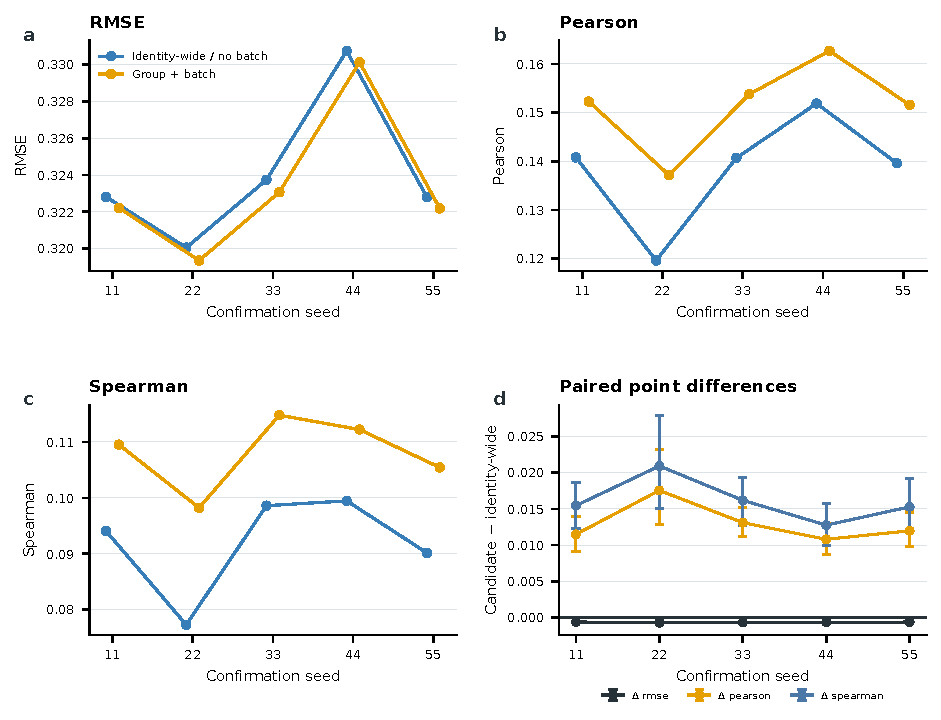
\includegraphics[width=\linewidth]{figures_batch/Fig2_cell_batch_repaired_performance.pdf}
\caption{\textbf{Locked confirmation under the frozen control reference.} Panels a--c show repaired RMSE, Pearson and Spearman values for the identity-wide/no-batch comparator and group-plus-batch candidate across the five confirmation seeds. Panel d shows paired candidate-minus-identity-wide point differences for the three metrics. The seed order is 11, 22, 33, 44 and 55; confirmation identities are scored once after validation-only penalty selection. Each point pools 36 held-out identities and 7,832--9,385 cells, depending on the split; the reported values are cell-by-gene aggregates, with no error bars in panels a--c and paired point differences in panel d.}
\label{fig:performance}
\end{figure}

\subsection{Identity-cluster uncertainty supports the paired advantage}
Cell-level scores contain many cells but the intervention identity is the independent unit for this prediction question. To avoid treating thousands of cells carrying one guide as independent biological replicates, we performed 2,000 paired bootstrap resamples of the held-out identity clusters within each repaired confirmation split. For every resample, all cells carrying a selected identity are included together for both models. The candidate-minus-identity-wide RMSE, Pearson and Spearman point differences are favorable in all five splits. With the corrected common-draw bootstrap, the identity-cluster sensitivity intervals for candidate-minus-identity-wide RMSE range from $[-0.00099,-0.00042]$, Pearson from $[0.00865,0.02324]$, and Spearman from $[0.00999,0.02792]$ across splits. These conditional intervals quantify the observed identity population; they do not provide biological replication.

These intervals answer a paired question: conditional on the observed Norman identity distribution, does adding the known gemgroup covariate improve cell-level prediction? They do not quantify variability across biological replicates, cell lines or independent screens. The same restriction applies to the five split-level standard deviations. The evidence is consistent with a local point-estimate direction and deliberately silent about broader transportability.



\subsection{Performance is retained for singleton and combination identities}
The identity split contains both singleton perturbations and combinations. A candidate that improves only because combination identities are overrepresented would have limited practical value, so we stratified the locked confirmation scores by identity composition. Across the five seeds, the batch-conditioned model improves RMSE in both strata. For singleton identities, the five-seed mean RMSE changes from 0.31665 to 0.31599, Pearson from 0.09760 to 0.11479 and Spearman from 0.06352 to 0.08373. For combination identities, the corresponding RMSE changes from 0.33391 to 0.33331, Pearson from 0.17442 to 0.18468 and Spearman from 0.12446 to 0.13662; the absolute errors are larger than for singleton identities. The heatmap in Fig.~\ref{fig:strata} shows a negative RMSE difference for every seed and both strata.

The combination result has a specific interpretation. Components of a combination may be seen as singles in training, but the complete combination identity is held out as one unit. The candidate therefore uses component indicators and pathway scores to form a compositional input while still being evaluated on an unseen complete label. It does not memorize a combination-specific response mean. The improvement in this stratum is consistent with a batch adjustment that acts on cells after the identity representation has been formed, rather than with a lookup of the combination label.

\begin{figure}[t]
\centering
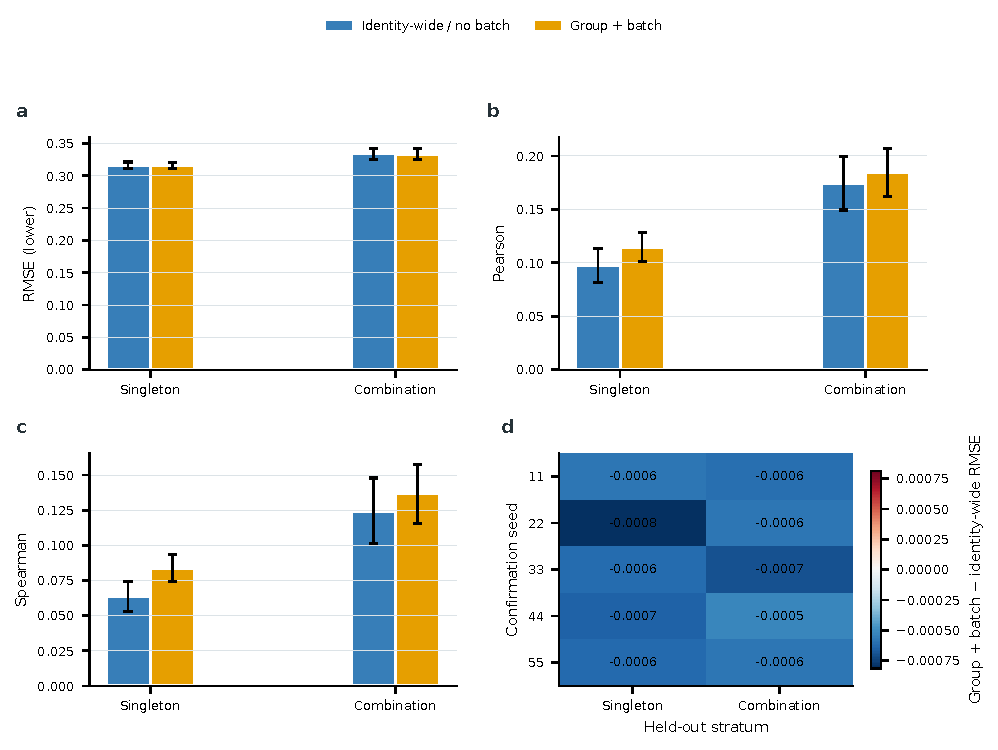
\includegraphics[width=\linewidth]{figures_batch/Fig3_cell_batch_strata.pdf}
\caption{\textbf{Composition-stratified confirmation under the frozen control reference.} Panels a--c compare RMSE, Pearson and Spearman for singleton and combination identities. Error bars are standard deviations across the five locked identity splits; each split pools 11--17 singleton identities and 3,171--6,425 cells or 19--25 combination identities and 2,795--4,661 cells. Panel d reports paired candidate-minus-baseline RMSE for each seed and stratum; every cell is negative. These are split-level summaries of the same confirmation protocol, not additional independent datasets.}
\label{fig:strata}
\end{figure}

\subsection{Component indicators carry the largest ablation signal}
The identity representation contains 512 panel-gene indicators, 256 pathway scores and 102 component indicators. A validation-only ablation removed one block at a time while keeping the frozen control reference, group-plus-batch fitting rule and penalty grid fixed. The component removal produced the largest and most consistent validation loss across the five seeds, whereas pathway and panel-gene removals were smaller and split dependent (Fig.~\ref{fig:ablation}). This is predictive sensitivity of the input contract; it does not establish a biological mechanism for any feature block.

\begin{figure}[t]
\centering
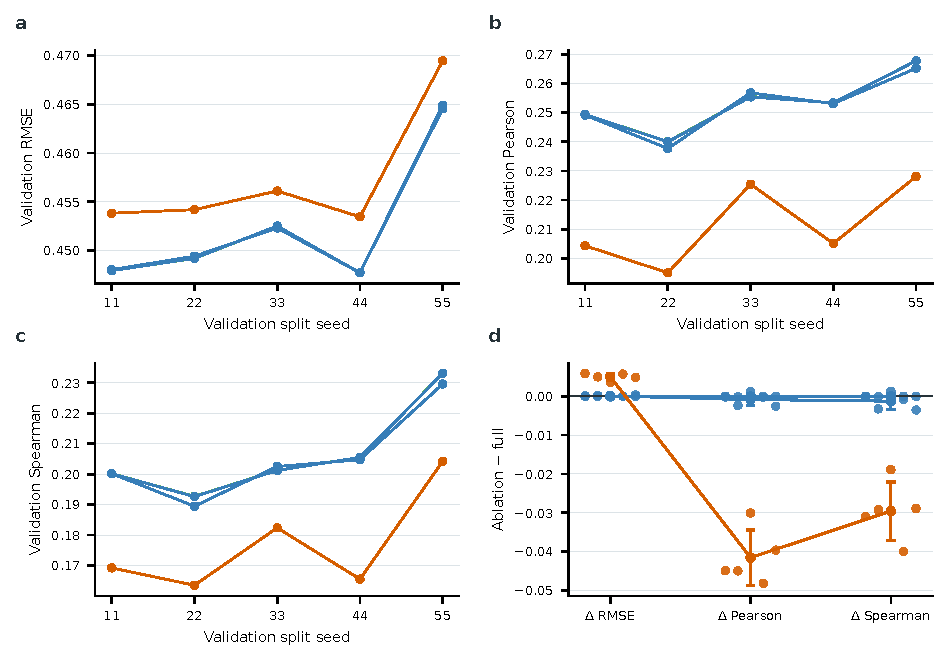
\includegraphics[width=\linewidth]{figures_batch/Fig4_cell_batch_ablation_repaired.pdf}
\caption{\textbf{Validation-only feature-block ablation under the frozen control reference.} Panels a--c show the five validation splits for the full group-plus-batch model and the three block-removal variants. Panel d shows paired ablation-minus-full changes for RMSE, Pearson and Spearman; points are individual validation seeds and bars are split standard deviations across five validation partitions (6,956--8,156 cells per partition). The component-indicator removal is the largest validation degradation. Confirmation targets are not used for this analysis, and the ablation is predictive sensitivity rather than a mechanistic attribution.}
\label{fig:ablation}
\end{figure}

\clearpage
\begin{figure}[p]
\centering
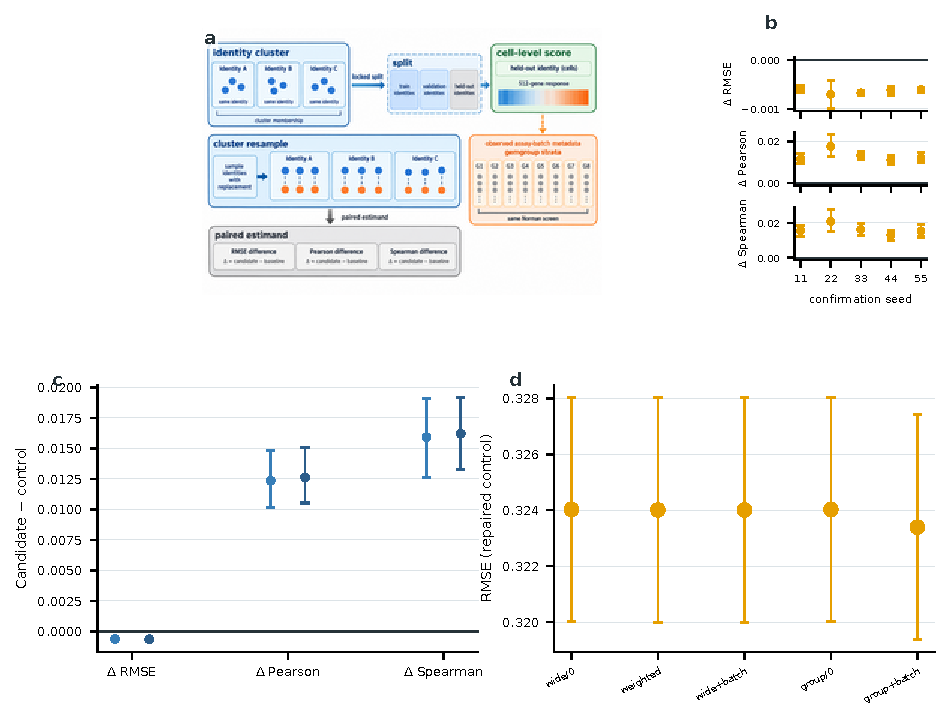
\includegraphics[width=\linewidth]{figures_batch/Fig5_identity_cluster_uncertainty_repaired.pdf}
\caption{\textbf{Identity-cluster uncertainty and aggregation controls.} Panel a is a conceptual schematic: complete identity clusters define the locked split and bootstrap unit, cell-level scores remain paired, and gemgroup is an observed assay-batch stratum within the same Norman screen. Panel b gives identity-cluster fixed-rank sensitivity intervals for candidate-minus-identity-wide RMSE, Pearson and Spearman differences (2,000 resamples; cells within an identity remain together). Panel c compares the candidate with aggregation-matched controls without the batch block for all three paired estimands, including Spearman intervals. Panel d reports the repaired aggregation-by-metadata factorial across five splits; points are split means and error bars are split standard deviations across the five locked identity partitions. Panel b uses 2,000 identity-cluster fixed-rank sensitivity resamples per split; panel c uses the same identity-cluster unit for paired sensitivity intervals. No panel represents independent biological replicates or external batch transfer.}
\label{fig:uncertainty}
\end{figure}
\clearpage

\subsection{Technical-batch availability and scope}
The eight gemgroups are known assay-batch metadata in the same Norman screen. Each contains 235--236 of the 236 non-control identities, and the smallest pairwise identity overlap is 235. Thus the screen supports within-screen comparison of observed gemgroups, but it does not provide an unseen batch coefficient for a strict leave-one-gemgroup-out deployment test. We therefore treat the batch-stratified panel as descriptive and restrict the claim to cells whose gemgroup is observed in this screen. Missing labels or a new experiment require a declared fallback or harmonization and are outside the present estimand.

The identity-held-out design prevents identity lookup: a complete combination can share components with training identities, but its full label is absent from fitting. The five confirmation splits improve all three point metrics, while the corrected paired identity-cluster sensitivity intervals remain conditional on one screen and one sampled identity population. The factorial shows that the complete aggregation-plus-metadata contract carries the point gain; the data do not identify a standalone gemgroup main effect. The candidate still leaves substantial residual variation (mean RMSE 0.3234), and the intervals are sensitivity summaries for paired split comparisons rather than per-cell prediction intervals.

\subsection{External transfer remains an unresolved boundary}
We performed a separate dataset-level transfer diagnostic using a common response map across Norman, Adamson and Dixit archives. The external mixing weight and ridge penalty were selected on validation identities only, followed by one locked transfer score. Across five repeated validation partitions, the selected external weight was zero in three partitions; the remaining partitions selected 0.05 or 0.5. On the one locked transfer score, the transfer mixture had a small RMSE decrease but did not improve Pearson and Spearman simultaneously under the prespecified all-metrics gate. These results are negative or indeterminate boundary evidence rather than a transfer claim. Differences in guide design, controls, cell context and response distributions prevent treating the within-Norman gemgroup result as cross-screen generalization.

\subsection{Locked retrospective intervention prioritization is enriched but unstable at the candidate level}
The response predictor was evaluated as a bounded decision aid for selecting combinations for follow-up assays. Before reading any locked response, we fixed the hit definition as the top-$k$ combinations by observed 512-gene response energy, the ranking score as predicted response energy, the list sizes $k\in\{5,10,20\}$, and the null overlap as $k/27$. For each identity partition, the ridge penalty was selected by validation-profile RMSE; the model then scored the 27 untouched combination identities once. This is a retrospective endpoint analysis within one Norman screen, not a prospective target-discovery or causal efficacy test.

On the locked combinations, mean top-$k$ overlap was 0.60, 0.76 and 0.89 for $k=5$, $10$ and $20$, compared with random nulls $k/27=0.185,0.370,0.741$; the corresponding enrichment ratios were 3.24, 2.05 and 1.20 (Table~\ref{tab:priority}). Mean NDCG was 0.867, 0.901 and 0.935. Predicted and observed response-energy ranks had Spearman correlation $0.727\pm0.085$ across the five identity partitions. Projection to the 256 fixed Reactome modules gave pathway Spearman $0.846\pm0.009$ and cosine similarity $0.901\pm0.018$. The displayed values summarize split means and split standard deviations; paired identity-cluster bootstrap sensitivity intervals (B=2,000, with common draws across $k$ and endpoints) are provided in Supplementary Table~\ref{tab:priority_bootstrap}.

Selected-label overlap was low under this protocol: mean pairwise Jaccard overlap across the five locked lists was 0.056 at top-$5$, 0.089 at top-$10$ and 0.114 at top-$20$. The candidate sets differ between identity partitions, so this is a joint partition and priority stability diagnostic rather than a pure ranking-repeatability estimate. The locked analysis supports a larger assay shortlist and pathway-level checking, while a single top-ranked combination should not be treated as a stable target. The earlier validation-only analysis is retained as exploratory context, but all application-facing numbers and captions now refer to the locked 27-combination evaluation.

\begin{table}[H]
\centering
\scriptsize
\caption{Locked retrospective intervention-priority evaluation. The penalty is selected by validation-profile RMSE and the 27 locked combinations are scored once. Top-$k$ overlap is the fraction of predicted top-$k$ labels that overlap the top-$k$ labels defined by locked observed response energy. The null overlap is $k/27$ and enrichment is observed overlap divided by this null. NDCG uses the locked observed-energy ordering, assay fraction is $k/27$, and Jaccard is the mean pairwise overlap of selected labels across the five identity partitions. Values are means across seeds; split standard deviations are shown in parentheses.}
\begin{tabular}{lcccccc}
\toprule
$k$ & Top-$k$ overlap & NDCG & Assay fraction & Null overlap & Enrichment & Jaccard \\
\midrule
5  & 0.600 (0.245) & 0.867 (0.090) & 18.5\% & 0.185 & 3.24 & 0.056 \\
10 & 0.760 (0.114) & 0.901 (0.037) & 37.0\% & 0.370 & 2.05 & 0.089 \\
20 & 0.890 (0.042) & 0.935 (0.024) & 74.1\% & 0.741 & 1.20 & 0.114 \\
\bottomrule
\end{tabular}
\label{tab:priority}
\end{table}

\begin{figure}[H]
\centering
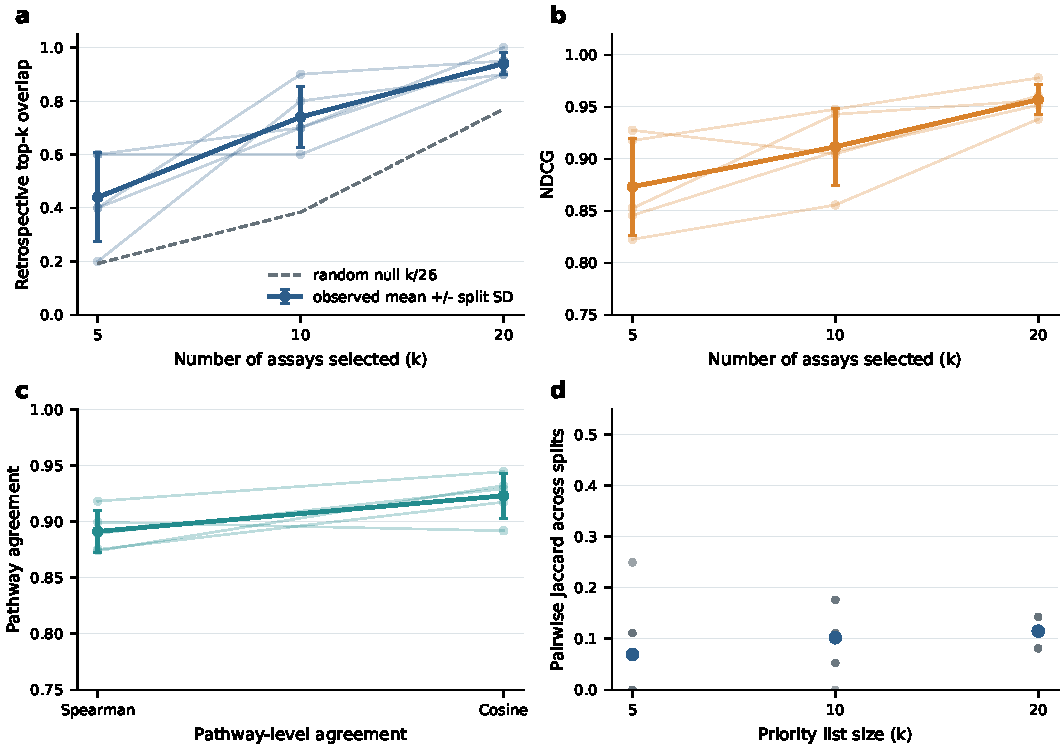
\includegraphics[width=\linewidth]{figures_batch/Fig6_intervention_priority.pdf}
\caption{\textbf{Locked retrospective intervention-priority evaluation.} Panel a shows top-$k$ overlap between predicted and locked observed-energy combinations; the dashed line is the random $k/27$ null. Panel b gives NDCG against locked observed response-energy ranks. Panel c shows pathway-profile Spearman and cosine similarity after projection to 256 Reactome modules. Panel d shows pairwise Jaccard overlap of selected identity labels across the five partition-specific locked lists; because candidate sets differ, this is a joint partition and priority stability diagnostic. Each split selects the penalty by validation-profile RMSE and scores 27 locked combinations once. Error bars in all panels are split standard deviations across the five seeds; the paired B=2,000 identity-cluster percentile sensitivity intervals use a common draw matrix within each seed and are reported in Supplementary Table~\ref{tab:priority_bootstrap}. The panels quantify retrospective ranking enrichment and pathway consistency, not clinical benefit, causal efficacy or external validation.}
\label{fig:priority}
\end{figure}

\begin{table}[ht]\centering\scriptsize\caption{Supplementary Table 3. Identity-cluster bootstrap sensitivity intervals for the locked priority endpoints. Each row is one locked identity partition; B=2,000 paired draws use a common draw matrix across k and endpoints. Values are percentile intervals. These intervals are sensitivity summaries for the observed screen and are distinct from the split standard deviations shown in Fig.~6 and Table~2.}\label{tab:priority_bootstrap}\begin{tabular}{rccccl}\toprule Seed & k & Overlap point [95\% interval] & NDCG point [95\% interval] & Energy Spearman point [95\% interval] \\ \midrule
11 & 5 & 0.826 [0.400, 1.000] & 0.963 [0.829, 1.000] & 0.695 [0.340, 0.919] \\
11 & 10 & 0.766 [0.500, 1.000] & 0.942 [0.845, 0.998] & 0.695 [0.340, 0.919] \\
11 & 20 & 0.843 [0.700, 0.950] & 0.963 [0.915, 0.992] & 0.695 [0.340, 0.919] \\
22 & 5 & 0.443 [0.000, 0.800] & 0.875 [0.720, 0.990] & 0.752 [0.587, 0.877] \\
22 & 10 & 0.765 [0.500, 1.000] & 0.922 [0.823, 0.991] & 0.752 [0.587, 0.877] \\
22 & 20 & 0.842 [0.700, 1.000] & 0.939 [0.883, 0.980] & 0.752 [0.587, 0.877] \\
33 & 5 & 0.582 [0.200, 1.000] & 0.882 [0.772, 0.989] & 0.820 [0.633, 0.928] \\
33 & 10 & 0.772 [0.500, 1.000] & 0.920 [0.854, 0.987] & 0.820 [0.633, 0.928] \\
33 & 20 & 0.923 [0.800, 1.000] & 0.950 [0.910, 0.991] & 0.820 [0.633, 0.928] \\
44 & 5 & 0.400 [0.000, 0.800] & 0.745 [0.536, 0.922] & 0.686 [0.337, 0.906] \\
44 & 10 & 0.718 [0.500, 0.900] & 0.827 [0.678, 0.944] & 0.686 [0.337, 0.906] \\
44 & 20 & 0.882 [0.750, 1.000] & 0.905 [0.825, 0.965] & 0.686 [0.337, 0.906] \\
55 & 5 & 0.561 [0.200, 1.000] & 0.895 [0.757, 0.981] & 0.597 [0.269, 0.823] \\
55 & 10 & 0.580 [0.300, 0.800] & 0.906 [0.817, 0.958] & 0.597 [0.269, 0.823] \\
55 & 20 & 0.883 [0.750, 1.000] & 0.935 [0.877, 0.974] & 0.597 [0.269, 0.823] \\
\bottomrule\end{tabular}\end{table}


\subsection{Matched nonlinear evidence remains unresolved}
A matched nonlinear comparison was attempted with the same 878-dimensional input and 512-gene target. Implementation review identified a mismatch between the stated validation criterion and the loss used for early stopping, an incorrectly recorded checkpoint epoch, and unpaired resampling in the reported difference intervals. The resulting numerical comparisons are invalid and are excluded from the scientific evidence. Correcting those errors requires a new validation-only analysis and an explicit evaluation boundary because the earlier confirmation outcomes have already been inspected. The available results therefore do not yet establish superiority over a sufficiently tuned matched nonlinear comparator.

\subsection{Exact rank re-evaluation and uncertainty interpretation}
The production bootstrap uses global ranks followed by additive identity-cluster resampling. Because the resampled population can change rank order, we performed an exact reranking sensitivity audit on the seed-11 confirmation split. For 128 identity-cluster draws, one 512-gene mean profile was formed for each sampled identity and Spearman correlation was recomputed from those profiles for both estimators; RMSE and Pearson used the same paired draws. The candidate-minus-baseline Spearman mean was $-0.002669$ (percentile interval $[-0.006269,0.000370]$), compared with $-0.001774$ ($[-0.004872,0.000887]$) for the fixed-rank approximation. The comparable widths and shared direction support the terminology ``identity-cluster sensitivity interval''; this finite identity-mean check is not the cell-level primary estimand or a biological replicate.

The five-split intervals should therefore be read as conditional perturbations of the observed held-out identity population. They do not quantify new cells, guides, cell lines or screens, and they are not hypothesis tests or calibrated confidence intervals. Pearson and RMSE are likewise conditional on the frozen control reference and sampled panel; the all-seed gate is a descriptive confirmation rule.

\section{Methods}
\subsection{Data and deterministic sampling}
The primary data are the processed Norman--Weissman Perturb-seq screen distributed through the versioned scPerturb archive and linked to the original study \citep{pmid31395745}. The h5ad object includes a sparse count matrix, perturbation and guide annotations, gemgroup, cell-quality fields and the gene vocabulary. We read perturbation labels from the categorical observation field and retain the source row index for every sampled cell. A deterministic random generator with seed 17 samples cells within each parsed perturbation label. The allocation is proportional to label support with a minimum of eight cells per label and a global target of approximately 60,000 cells, producing the 59,879-cell panel used here. The sampling is performed once before any identity split and the resulting source indices are frozen for all five seeds.

The control parser treats missing-like strings (including ``nan'', ``*'' and ``None'') and explicit negative or control tokens as CONTROL. A label is otherwise split on the component delimiter, guide suffixes are removed by the parser and the remaining component names are joined in a canonical order. The audit found 11,855 raw control cells in the filtered object and 6,382 controls in the sampled panel. In the observed release, all raw control cells belong to the category ``control''; the parser rule remains explicit so that a future release cannot silently change the estimand. The repaired control mean uses the fixed even-source-row subset of 3,207 sampled CONTROL cells, frozen before identity splitting; the confirmation identities never contribute to this reference. Perturbation labels that contain two or more components remain one identity for splitting and evaluation.

\subsection{Output panel and identity features}
The output panel contains 512 genes fixed before the locked evaluation. For a cell, the panel array is extracted from the sparse count matrix, library-size normalized and log transformed. It is used as the response array after subtraction of the control mean. The panel names are also used as one of the identity feature vocabularies: if a perturbation targets one of these genes, the corresponding identity indicator is one. This dual naming does not leak endpoint expression because the feature value is derived from the perturbation label, while the measured expression appears only in the response array.

Reactome human pathway membership is represented by a gene-by-module matrix. We retain 256 modules after the fixed vocabulary and size filters and calculate a pathway score from the identity indicators and this fixed membership matrix. The 102 component indicators are binary features for component genes represented in the identity vocabulary. A combination therefore has a multi-hot component block and the corresponding union of pathway scores. The feature blocks are concatenated in the order identity panel genes, pathway scores and component indicators. The batch block is appended only for the candidate. No feature is computed from the target matrix, from a test cell's endpoint expression or from a cell-quality field.

\subsection{Control-relative response}
For every sampled cell, the normalized expression vector $x_i$ is centered by the control mean $\bar{x}_0$. This produces $y_i$ in the same 512-dimensional space as the output panel. The target is not an identity mean; every validation and confirmation cell contributes to the cell-level metric after the model has been trained on training identities. The fitting rows are identity means or identity-by-batch means, while the scoring rows remain individual cells. This separation allows a direct test of cell-level generalization without allowing a high-support identity to dominate model fitting.

The control subtraction is part of the estimand rather than a cosmetic plotting choice. If absolute expression were scored, a model could obtain a high correlation by predicting a shared housekeeping component. The control-relative response asks whether the predicted direction and magnitude of intervention-associated change agree with each observed cell. All reported RMSE values are in log-normalized expression units over the 512 output genes and the held-out cells. Pearson and Spearman correlations are calculated after flattening the corresponding cell-by-gene matrices. We do not combine the three metrics into one optimized score; the strict gate requires an improvement in all three.

\subsection{Identity-by-gemgroup fitting}
For each training identity $p$ and batch $b$, let $I_{pb}$ be the set of sampled cells with that identity and gemgroup. We retain a group when $|I_{pb}|\ge 2$. The candidate's training response is $\bar{y}_{pb}$ and its design row is the concatenation of $f_p$ and the batch one-hot vector for $b$. The identity-only comparator uses $\bar{y}_{p\cdot}$ and $f_p$. Both designs are standardized using training rows only. The same identity labels, output panel and control subtraction are used in both fits.

The ridge solution is calculated with a singular-value decomposition. This implementation is numerically stable when the 870 identity features are correlated and when the number of identity-by-batch rows is close to the feature dimension. The candidate has between 1,325 and 1,326 training group rows across the five splits. The baseline has one response row for each training identity, including the control row used to define the centered output. The penalty grid is selected on validation cells by RMSE; Pearson and Spearman are recorded but never used to select a penalty. The selected penalty and identity split are frozen before confirmation predictions are generated.

\subsection{Baselines and ablations}
The primary baseline is the identity-wide/no-batch ridge with the identical 870-dimensional perturbation representation and no gemgroup block. The candidate is not allowed extra pathway modules, extra output genes or response-derived covariates. The factorial controls described above hold either aggregation or metadata constant. The ablation variants remove pathway scores, panel-gene indicators or component indicators one block at a time while preserving the candidate's gemgroup block and fitting rule. These variants answer complementary questions: whether the explicit pathway prior contributes, whether output-panel identity labels contribute beyond components and pathways, and whether component-level composition carries information that the other blocks do not.

The estimator is deliberately linear. This keeps the primary comparison auditable without attributing a small gain to an unbounded increase in parameters. A matched MLP comparator was specified with the same 878-dimensional input and 512-dimensional target, but its first implementation used an inconsistent early-stopping criterion and invalid paired resampling; those outputs are retained as an implementation audit and excluded from the evidence. A corrected validation run is required before any nonlinear family claim.

\subsection{Pathway-level context decoder}
The pathway-level context result is an in-house neural additive decoder used to test whether a pathway-organized profile representation gives a comparable profile-level reference. It is separate from the primary cell-level batch-conditioned Ridge and receives no gemgroup covariate. For the fixed split with 165 training, 35 validation and 36 confirmation identities, the decoder uses 256 standardized pathway scores and 512 gene-panel indicators. Each pathway contributes a positive-gated rank-16 low-rank term and a direct pathway term; a gene residual and a 512-dimensional intercept are added to form the output. The implementation has 406,272 trainable parameters. Pathway features and gene-wise targets are standardized on training identities and transformed back to response units for scoring.

The decoder is optimized with AdamW (learning rate $7\times10^{-4}$ and weight decay $10^{-3}$), for at most 1,000 epochs with validation-loss early stopping after 70 non-improving epochs. Optimization seeds 11, 22 and 33 use the same split and are averaged only for the contextual summary. The reported Pathway-NEAT values are therefore three optimization runs on one profile-level estimand, not three independent splits or a matched comparator for the primary estimator. This in-house implementation is included to expose pathway-level context and is not presented as a newly validated clinical or mechanistic model.

\subsection{Metrics and uncertainty}
RMSE is the square root of the mean squared error across all confirmation cells and output genes. Pearson correlation measures flattened linear alignment and Spearman correlation measures rank alignment. The perturbation identity is the cluster unit for uncertainty. For each seed we resample the 36 held-out identities with replacement 2,000 times for both the repaired primary bundle and the aggregation factorial. The same draw indices are shared by every compared model, all cells carrying a selected identity are included together, and paired candidate-minus-control RMSE, Pearson and Spearman differences are recomputed. Spearman intervals use a fixed-rank sensitivity approximation: ranks are computed once on the locked observations and then resampled with the identity clusters. Because this approximation does not recompute ranks within every resample, the intervals are reported as sensitivity intervals rather than calibrated confidence limits. This procedure preserves within-identity cell dependence and the pairing of predictions from the compared estimators.

The five seeds are independent choices of identity partition and not independent experiments. We therefore report their mean and standard deviation as split sensitivity. The batch-stratified panel reports all eight gemgroups and the singleton/combination strata, but it does not treat those strata as additional biological cohorts. No p-value is assigned to the split-level mean. The all-seed gate is descriptive and was applied uniformly to the repaired confirmation run: each confirmation split must show lower RMSE and higher Pearson and Spearman correlation for the candidate. This was a retrospective computational analysis rather than a prospective preregistration.

\subsection{Exploration, confirmation and provenance}
Exploratory screens selected the input contract and estimator family using training and validation identities only. The locked confirmation run then fixed the control reference, complete-identity seeds, minimum supported-group size, seven-value alpha grid, aggregation factorial and three-metric all-seed gate; confirmation responses were not used to alter these choices. The input audit checked unique source rows and label agreement, eight observed gemgroups, disjoint identity partitions, the 512/256/102 feature blocks, the 512-gene output panel and exclusion of the response from the design. The lock audit and source digests are retained in the reproducibility bundle; they are provenance records rather than preregistration.

\subsection{Algorithmic and numerical specification}
After sparse extraction, the sampled output panel is stored as a dense $59{,}879\\times512$ float array; the genome-wide count object remains sparse. Identity features form a $237\\times870$ matrix (512 panel-gene indicators, 256 pathway scores and 102 component indicators), and appending the eight-level gemgroup one-hot gives 878 candidate columns. Training rows are accumulated by integer identity--gemgroup keys before the minimum-support rule is applied, preventing file order from changing row weights. Fits use a singular-value multi-output ridge solution with fitting-row standardization; scales below $10^{-3}$ are clipped to that floor. The validation search evaluates $0.1,1,3,10,30,100,300$, selects the smallest validation RMSE and resolves ties toward lower alpha. One coefficient matrix then scores all confirmation cells.

Primary correlations use row-major flattening of the same held-out cell-by-gene arrays for both estimators. Identity-cluster resampling retains complete cell slices and allows repeated identities, whereas the exact rank audit recomputes ranks from identity means; the production Spearman interval keeps locked global ranks and is explicitly a sensitivity approximation. Detailed source-row, panel, split and control-reference digests, per-seed denominators and software hashes remain in the machine-readable bundle rather than the reader-facing text.

\subsection{Intervention-priority simulation}
The prioritization analysis asks whether a predictor can enrich a fixed assay shortlist for large observed transcriptional responses. Its input is the same identity/pathway/component representation used for the pathway-level Ridge context, and its output is a scalar response-energy score derived from the predicted 512-gene control-relative profile. For each of the five identity partitions, all singleton identities were retained and two-component combinations were divided into 26 validation combinations and 27 locked combinations. The Ridge penalty was chosen by validation-profile RMSE using training identities; the locked combinations were then scored once. Before that score was read, the endpoint hit set, list sizes $k\in\{5,10,20\}$, and null overlap $k/27$ were fixed. No locked response was used for model, penalty or threshold selection.

For a locked combination $j$, predicted energy was $s_j=\sqrt{512^{-1}\sum_g\hat{y}_{jg}^{2}}$ and observed energy was computed by the same formula from the locked response profile. For each $k$, the retrospective hit set was the $k$ combinations with the highest locked observed energies within that split. We report top-$k$ overlap at $k\in\{5,10,20\}$, NDCG using the locked observed-energy ordering, the relative assay fraction $k/27$ and enrichment relative to the null overlap $k/27$. To assess biological organization without asserting mechanism, each 512-gene profile was projected to 256 fixed Reactome modules and compared by Spearman correlation and cosine similarity. Candidate identity stability was measured as the mean pairwise Jaccard overlap of the selected labels across the five seeds. For each endpoint we resampled the 27 locked identities with replacement 2,000 times while preserving all cells within an identity; these intervals are identity-cluster sensitivity summaries. Means and standard deviations are descriptive split summaries, and no prospective operating threshold or causal interpretation is assigned. The analysis is a CPU calculation on frozen arrays and was generated by the reproducible analysis bundle alongside the saved numerical result and quantitative figure.

\subsection{Reproducibility and estimand scope}
All computations use the frozen sampled panel and the same five identity seeds; the closed-form fit is deterministic once split and alpha are fixed. The design array contains perturbation identity features and observed gemgroup metadata, the response array contains the normalized 512-gene panel after subtraction of the frozen 3,207-cell control reference, and the split index records complete identities. Only the design array enters fitting; the response is used for validation, confirmation and the locked prioritization analysis. The fixed control reference and training-only standardization make the target comparable across splits, while the reported estimand remains conditional on this screen's control composition.

A training identity contributes one identity-wide row to the baseline or one supported identity--gemgroup row to the candidate, with at least two cells per retained group; every eligible held-out cell contributes to scoring. The five seeds are partition sensitivities rather than biological replicates, strata are not extra cohorts, and no p-value is assigned to their mean. The observed gemgroup is a known within-Norman assay label: its eight levels overlap 235--236 of 236 non-control identities, so the design does not identify an unseen-batch coefficient or justify arbitrary leave-one-gemgroup-out imputation. New screens require a declared encoding and harmonization map before transfer can be evaluated.

\section{Discussion}
The central result is bounded: under an independently frozen control reference, the group-plus-batch ridge has favorable RMSE, Pearson and Spearman point estimates in all five identity-held-out splits. The RMSE change is small, while the correlation changes are larger. Corrected paired identity-cluster sensitivity intervals remain conditional on one screen and one sampled identity population. The aggregation factorial shows that the complete group-and-batch contract carries the point gain; the data do not identify a standalone gemgroup main effect.

The retrospective prioritization analysis gives the prediction task a concrete experimental use without changing its estimand. Response-energy ranking enriched the observed high-response set and preserved pathway-level agreement, but the low cross-seed Jaccard values show that shortlist identity is sensitive to the held-out partition. The appropriate operational interpretation is therefore a ranked assay shortlist whose pathway-level pattern can be checked, rather than a single computationally established target. Because the analysis is a retrospective endpoint evaluation within one Norman screen and the shortlist identity is unstable across held-out partitions, it does not establish prospective enrichment, therapeutic value or causal pathway action.

The result also clarifies what the model is learning. The baseline averages a training identity over all observed batches. The candidate estimates identity-by-gemgroup rows and can shift a prediction toward the technical distribution expected for the queried cell. The eight indicators are known assay-batch metadata, not biological labels, and should not be interpreted as pathway activity. The appropriate reading is therefore a conditional prediction statement within this Norman screen; the factorial does not support attributing the gain to a batch coefficient alone.

The claim is conditional on the cell-level Norman contract: complete identities are held out, but the target is centered by one frozen control reference and the observed gemgroup is an in-screen technical label. Norman, Adamson and Dixit differ in guide design, controls, sequencing and context, so no transfer across archives or cell lines is established; an external study would need a predeclared experiment-level split and harmonization map.

The model is also not a causal pathway simulator, consistent with prior discussions of pathway annotation uncertainty \citep{pmid21199820}. Its Reactome scores are deterministic functions of the perturbation identity, and its coefficients quantify conditional predictive associations. This distinction follows the broader single-cell analysis literature, where clustered cells, pseudobulk summaries and replicate-aware tests are required for calibrated uncertainty \citep{luecken2022,hao2021,kiselev2018,lun2016,benjamini1995,mccarthy2012}. A module can be predictive because it shares genes with a response program, because it encodes a useful prior for combinations or because it correlates with an unmeasured technical factor. No coefficient alone demonstrates pathway activation. Post-hoc attribution tools such as SHAP and integrated gradients can describe a fitted predictor, but they do not convert an association into an intervention effect \citep{lundberg2017,sundararajan2017}. Causal interpretation would require perturbation-specific controls, temporal measurements, orthogonal assays and interventions that break the relevant confounding. The current evidence supports an auditable predictive decomposition, not mechanistic discovery.

The modest model size is a strength for auditing. The same design can be implemented with a different linear penalty, a low-rank decoder or a neural architecture without changing the estimand. A future nonlinear method should report parameter count, nested validation, identity-cluster uncertainty and a control with matched input dimensionality. It should also test whether the component-indicator channel remains necessary and whether its gain persists when gemgroup labels are masked or when the evaluation is moved to a new experiment. The present ridge model provides the operating baseline against which those additions can be judged.

\section{Limitations and future work}
The analysis uses one primary cell line and one public screen. Even though five identity partitions are evaluated, they are not five independent biological replicates. The 512-gene output panel is fixed and may omit responses that are important for a particular perturbation. The Reactome vocabulary is curated and incomplete, and the 102 component indicators reflect the observed identity vocabulary rather than all possible gene combinations. Gemgroup is a coarse technical label; within-batch variation, guide efficacy, cell cycle and quality effects remain unmodeled. Identity-by-batch groups with fewer than two cells are excluded from the fitting rows, although their cells remain eligible for confirmation scoring. These constraints define the population to which the current metrics apply.

A useful extension would fit a hierarchical model that separates identity, batch and identity-by-batch interaction while retaining identity-held-out confirmation. Such a model could propagate uncertainty from sparse groups and quantify whether a batch effect is shared across perturbations or concentrated in a subset. Another extension would add calibration curves for predicted response magnitude and conformal intervals evaluated on held-out identities. A multi-archive study could test whether gemgroup metadata transfers after a declared harmonization map. The attempted matched MLP comparison remains unresolved after implementation errors; a future neural or foundation-model predictor would need a prespecified architecture, nested validation, identity-cluster uncertainty and improvement over the ridge on all three metrics across independent experiments.

\section*{Author information and declarations}
\textbf{Author contributions.} The submitting authors will complete the CRediT contribution statement before submission; the current analysis was conducted as a single-team computational study.\\
\textbf{Funding.} No external funding source was used for this computational analysis; final grant identifiers, if applicable, will be supplied by the submitting authors.\\
\textbf{Acknowledgements.} The authors will add acknowledgements for data custodians and infrastructure support in the submission package.\\
\textbf{Competing interests.} The authors declare no competing interests.\\
\textbf{Ethics declarations.} This study reanalyses public, de-identified data and collected no new human or animal material; no additional institutional review was required for this computational reanalysis.

\section{Data Availability}
The Norman--Weissman Perturb-seq source experiment is publicly available through the scPerturb archive and GEO series GSE133344, the original study accession \citep{pmid31395745}. Reactome annotations are available from the Reactome project \citep{reactome2020}. The frozen processed panel, numerical result objects, figure sources and provenance manifests are released at the public versioned archive https://github.com/jinluo12345/norman-perturbseq-identity-ridge/tree/v1.1.5. Raw h5ad files remain available from GSE133344; the release records their source checksums rather than duplicating them.

\section{Code Availability}
The custom analysis and figure-generation code, numerical result objects, figure sources, native image2 provenance, panel manifest and pinned environment are deposited at https://github.com/jinluo12345/norman-perturbseq-identity-ridge/tree/v1.1.5. The tag is the immutable release reference used for this manuscript; the repository's commit history and SHA-256 manifest provide version and file integrity checks.

\section{Reporting summary}
This is a retrospective computational analysis of public single-cell perturbation data with no new human or animal material. The prediction unit is a cell, the fitting unit is an identity or identity-by-gemgroup group, and the uncertainty unit is a held-out perturbation identity; model choices use training and validation identities only.

\begin{thebibliography}{51}
\providecommand{\natexlab}[1]{#1}
\providecommand{\url}[1]{\texttt{#1}}
\expandafter\ifx\csname urlstyle\endcsname\relax
  \providecommand{\doi}[1]{doi: #1}\else
  \providecommand{\doi}{doi: \begingroup \urlstyle{rm}\Url}\fi

\bibitem[Dixit et~al.(2016)]{dixit2016}
Abhimanyu Dixit et~al.
\newblock Perturb-seq: dissecting molecular circuits with scalable single-cell
  rna profiling of pooled genetic screens.
\newblock \emph{Cell}, 167:\penalty0 1853--1866, 2016.
\newblock \doi{10.1016/j.cell.2016.11.038}.

\bibitem[Adamson et~al.(2016)]{adamson2016}
Britt Adamson et~al.
\newblock A multiplexed single-cell crispr screening platform enables
  systematic dissection of the unfolded protein response.
\newblock \emph{Cell}, 167:\penalty0 1867--1882, 2016.
\newblock \doi{10.1016/j.cell.2016.11.048}.

\bibitem[Datlinger et~al.(2017)]{datlinger2017}
P.~Datlinger et~al.
\newblock Pooled crispr screening with single-cell transcriptome readout.
\newblock \emph{Nature Methods}, 14:\penalty0 297--301, 2017.
\newblock \doi{10.1038/nmeth.4177}.

\bibitem[Gasperini et~al.(2019)]{gasperini2019}
M.~Gasperini et~al.
\newblock A genome-wide framework for mapping gene regulation via cellular
  genetic screens.
\newblock \emph{Nature}, 567:\penalty0 354--358, 2019.
\newblock \doi{10.1038/s41586-019-1369-3}.

\bibitem[McFaline-Figueroa et~al.(2019)]{mcfalinefigueroa2019}
J.~L. McFaline-Figueroa et~al.
\newblock A pooled single-cell genetic screen identifies regulatory checkpoints
  in the fate of embryonic stem cells.
\newblock \emph{Nature Methods}, 16:\penalty0 387--395, 2019.
\newblock \doi{10.1038/s41592-019-0427-2}.

\bibitem[Schraivogel et~al.(2020)]{schraivogel2020}
D.~Schraivogel et~al.
\newblock Targeted perturb-seq enables genome-scale genetic screens in single
  cells.
\newblock \emph{Nature Methods}, 17:\penalty0 629--635, 2020.
\newblock \doi{10.1038/s41587-020-0478-1}.

\bibitem[Replogle et~al.(2020)]{pmid32231336}
Joseph~M. Replogle et~al.
\newblock Combinatorial single-cell crispr screens by direct guide rna capture
  and targeted sequencing.
\newblock \emph{Nature biotechnology}, 38\penalty0 (8):\penalty0 954--961,
  2020.

\bibitem[Replogle et~al.(2022{\natexlab{a}})]{pmid35688146}
Joseph~M. Replogle et~al.
\newblock Mapping information-rich genotype-phenotype landscapes with
  genome-scale perturb-seq.
\newblock \emph{Cell}, 185\penalty0 (14):\penalty0 2559--2575.e28,
  2022{\natexlab{a}}.

\bibitem[Replogle et~al.(2022{\natexlab{b}})]{replogle2022}
Joseph~M. Replogle et~al.
\newblock A de novo noncoding rna screen in human cells.
\newblock \emph{Science}, 377:\penalty0 eabp8870, 2022{\natexlab{b}}.
\newblock \doi{10.1126/science.abp8870}.

\bibitem[Lotfollahi et~al.(2019)]{lotfollahi2019}
Mohammad Lotfollahi et~al.
\newblock scgen predicts single-cell perturbation responses.
\newblock \emph{Nature Methods}, 16:\penalty0 715--721, 2019.
\newblock \doi{10.1038/s41592-019-0494-8}.

\bibitem[Lotfollahi et~al.(2020)]{lotfollahi2020}
Mohammad Lotfollahi et~al.
\newblock Compositional perturbation autoencoder for single-cell response
  modeling.
\newblock \emph{Nature Methods}, 17:\penalty0 1096--1106, 2020.
\newblock \doi{10.1038/s41592-020-00940-4}.

\bibitem[Roohani et~al.(2023)]{roohani2023}
Yasin Roohani et~al.
\newblock Predicting transcriptional outcomes of novel multigene perturbations
  with gears.
\newblock \emph{Nature Biotechnology}, 41:\penalty0 1357--1366, 2023.
\newblock \doi{10.1038/s41587-023-01905-6}.

\bibitem[Lopez et~al.(2018)Lopez, Regier, Cole, Jordan, and Yosef]{lopez2018}
R.~Lopez, J.~Regier, M.~B. Cole, M.~I. Jordan, and N.~Yosef.
\newblock Deep generative modeling for single-cell transcriptomics.
\newblock \emph{Nature Methods}, 15:\penalty0 1053--1058, 2018.
\newblock \doi{10.1038/s41592-018-0229-2}.

\bibitem[Lotfollahi et~al.(2022)]{lotfollahi2022}
M.~Lotfollahi et~al.
\newblock Mapping single-cell data to reference atlases by transfer learning.
\newblock \emph{Nature Biotechnology}, 40:\penalty0 121--130, 2022.
\newblock \doi{10.1038/s41587-021-01001-7}.

\bibitem[Theodoris et~al.(2023)]{geneformer2023}
Christina~V. Theodoris et~al.
\newblock Transfer learning enables predictions in network biology.
\newblock \emph{Nature}, 618:\penalty0 616--624, 2023.
\newblock \doi{10.1038/s41586-023-06139-9}.

\bibitem[Osorio et~al.(2022)]{pmid35510185}
D.~Osorio et~al.
\newblock sctenifoldknk: An efficient virtual knockout tool for gene function
  predictions via single-cell gene regulatory network perturbation.
\newblock \emph{Patterns (New York, N.Y.)}, 3\penalty0 (3):\penalty0 100434,
  2022.

\bibitem[Lotfollahi et~al.(2023)]{pmid37154091}
Mohammad Lotfollahi et~al.
\newblock Predicting cellular responses to complex perturbations in
  high-throughput screens.
\newblock \emph{Molecular systems biology}, 19\penalty0 (6):\penalty0 e11517,
  2023.

\bibitem[Ji et~al.(2021)]{pmid34139164}
Y.~Ji et~al.
\newblock Machine learning for perturbational single-cell omics.
\newblock \emph{Cell systems}, 12\penalty0 (6):\penalty0 522--537, 2021.

\bibitem[Joung et~al.(2023)]{pmid36608654}
J.~Joung et~al.
\newblock A transcription factor atlas of directed differentiation.
\newblock \emph{Cell}, 186\penalty0 (1):\penalty0 209--229.e26, 2023.

\bibitem[Kamimoto et~al.(2023)]{pmid36755098}
K.~Kamimoto et~al.
\newblock Dissecting cell identity via network inference and in silico gene
  perturbation.
\newblock \emph{Nature}, 614\penalty0 (7949):\penalty0 742--751, 2023.

\bibitem[Hao et~al.(2024)]{pmid38844628}
M.~Hao et~al.
\newblock Large-scale foundation model on single-cell transcriptomics.
\newblock \emph{Nature methods}, 21\penalty0 (8):\penalty0 1481--1491, 2024.

\bibitem[Ahlmann-Eltze et~al.(2025)]{pmid40759747}
C.~Ahlmann-Eltze et~al.
\newblock Deep-learning-based gene perturbation effect prediction does not yet
  outperform simple linear baselines.
\newblock \emph{Nature methods}, 22\penalty0 (8):\penalty0 1657--1661, 2025.

\bibitem[Yang et~al.(2022)]{scbert2022}
F.~Yang et~al.
\newblock scbert as a large-scale pretrained deep language model for cell type
  annotation of single-cell rna-seq data.
\newblock \emph{Nature Machine Intelligence}, 4:\penalty0 852--866, 2022.
\newblock \doi{10.1038/s42256-021-00449-9}.

\bibitem[Qi et~al.(2024)Qi, Zhao, Tian, Li, Chen, et~al.]{qi2024}
Xiaoning Qi, Lianhe Zhao, Chenyu Tian, Yueyue Li, Zhen-Lin Chen, et~al.
\newblock Predicting transcriptional responses to novel chemical perturbations
  using deep generative model for drug discovery.
\newblock \emph{Nature Communications}, 15\penalty0 (1), 2024.
\newblock \doi{10.1038/s41467-024-53457-1}.

\bibitem[Tian et~al.(2019)]{pmid31422865}
R.~Tian et~al.
\newblock Crispr interference-based platform for multimodal genetic screens in
  human ipsc-derived neurons.
\newblock \emph{Neuron}, 104\penalty0 (2):\penalty0 239--255.e12, 2019.

\bibitem[Jin et~al.(2020)]{pmid33243861}
X.~Jin et~al.
\newblock In vivo perturb-seq reveals neuronal and glial abnormalities
  associated with autism risk genes.
\newblock \emph{Science (New York, N.Y.)}, 370\penalty0 (6520), 2020.

\bibitem[Zheng et~al.(2024)]{pmid38772369}
X.~Zheng et~al.
\newblock Massively parallel in vivo perturb-seq reveals cell-type-specific
  transcriptional networks in cortical development.
\newblock \emph{Cell}, 187\penalty0 (13):\penalty0 3236--3248.e21, 2024.

\bibitem[Rothfels et~al.(2023)]{pmid37053306}
K.~Rothfels et~al.
\newblock Using the reactome database.
\newblock \emph{Current protocols}, 3\penalty0 (4):\penalty0 e722, 2023.

\bibitem[Wolf et~al.(2018)Wolf, Angerer, and Theis]{wolf2018}
F.~A. Wolf, P.~Angerer, and F.~J. Theis.
\newblock Scanpy: large-scale single-cell gene expression data analysis.
\newblock \emph{Genome Biology}, 19:\penalty0 15, 2018.
\newblock \doi{10.1186/s13059-017-1382-0}.

\bibitem[Stuart et~al.(2019)]{stuart2019}
T.~Stuart et~al.
\newblock Comprehensive integration of single-cell data.
\newblock \emph{Cell}, 177:\penalty0 1888--1902, 2019.
\newblock \doi{10.1016/j.cell.2019.05.031}.

\bibitem[Haghverdi et~al.(2018)Haghverdi, Lun, Morgan, and
  Marioni]{haghverdi2018}
L.~Haghverdi, A.~T.~L. Lun, M.~D. Morgan, and J.~C. Marioni.
\newblock Batch effects in single-cell rna-sequencing data are corrected by
  matching mutual nearest neighbors.
\newblock \emph{Nature Biotechnology}, 36:\penalty0 421--427, 2018.
\newblock \doi{10.1038/nbt.4091}.

\bibitem[Korsunsky et~al.(2019)]{korsunsky2019}
I.~Korsunsky et~al.
\newblock Fast, sensitive and accurate integration of single-cell data with
  harmony.
\newblock \emph{Nature Methods}, 16:\penalty0 1289--1296, 2019.
\newblock \doi{10.1038/s41592-019-0619-0}.

\bibitem[Gayoso et~al.(2022)]{gayoso2021}
A.~Gayoso et~al.
\newblock scvi-tools: a library for deep probabilistic analysis of single-cell
  omics data.
\newblock \emph{Nature Biotechnology}, 40:\penalty0 163--166, 2022.
\newblock \doi{10.1038/s41587-021-01206-w}.

\bibitem[Mimitou et~al.(2019)]{mimitou2019}
E.~P. Mimitou et~al.
\newblock Scalable, multimodal profiling of chromatin accessibility, gene
  expression and protein levels in single cells.
\newblock \emph{Nature Methods}, 16:\penalty0 1246--1253, 2019.
\newblock \doi{10.1038/s41592-019-0460-6}.

\bibitem[Stoeckius et~al.(2017)]{stoeckius2017}
M.~Stoeckius et~al.
\newblock Simultaneous epitope and transcriptome measurement in single cells.
\newblock \emph{Nature Methods}, 14:\penalty0 865--868, 2017.
\newblock \doi{10.1038/nmeth.4380}.

\bibitem[Cao et~al.(2017)]{cao2018}
J.~Cao et~al.
\newblock Comprehensive single-cell transcriptional profiling of a
  multicellular organism.
\newblock \emph{Science}, 357:\penalty0 661--667, 2017.
\newblock \doi{10.1126/science.aam8940}.

\bibitem[Andreatta et~al.(2021)]{pmid34017005}
M.~Andreatta et~al.
\newblock Interpretation of t cell states from single-cell transcriptomics data
  using reference atlases.
\newblock \emph{Nature communications}, 12\penalty0 (1):\penalty0 2965, 2021.

\bibitem[Squair et~al.(2021)]{pmid34584091}
J.~W. Squair et~al.
\newblock Confronting false discoveries in single-cell differential expression.
\newblock \emph{Nature communications}, 12\penalty0 (1):\penalty0 5692, 2021.

\bibitem[Gillespie et~al.(2022)]{reactome2020}
Marc Gillespie et~al.
\newblock The reactome pathway knowledgebase.
\newblock \emph{Nucleic Acids Research}, 50:\penalty0 D687--D692, 2022.
\newblock \doi{10.1093/nar/gkab1028}.

\bibitem[Fabregat et~al.(2018)]{pmid29377902}
Antonio Fabregat et~al.
\newblock Reactome graph database: Efficient access to complex pathway data.
\newblock \emph{PLoS computational biology}, 14\penalty0 (1):\penalty0
  e1005968, 2018.

\bibitem[Jupe et~al.(2018)]{pmid29378288}
S.~Jupe et~al.
\newblock Interleukins and their signaling pathways in the reactome biological
  pathway database.
\newblock \emph{The Journal of allergy and clinical immunology}, 141\penalty0
  (4):\penalty0 1411--1416, 2018.

\bibitem[Norman et~al.(2019)]{pmid31395745}
Thomas~M. Norman et~al.
\newblock Exploring genetic interaction manifolds constructed from rich
  single-cell phenotypes.
\newblock \emph{Science (New York, N.Y.)}, 365\penalty0 (6455):\penalty0
  786--793, 2019.

\bibitem[Dall'Olio et~al.(2011)]{pmid21199820}
G.~M. Dall'Olio et~al.
\newblock The annotation of the asparagine n-linked glycosylation pathway in
  the reactome database.
\newblock \emph{Glycobiology}, 21\penalty0 (11):\penalty0 1395--400, 2011.

\bibitem[Luecken et~al.(2022)]{luecken2022}
M.~D. Luecken et~al.
\newblock Benchmarking atlas-level data integration in single-cell genomics.
\newblock \emph{Nature Methods}, 19:\penalty0 41--50, 2022.
\newblock \doi{10.1038/s41592-021-01336-8}.

\bibitem[Hao et~al.(2021)]{hao2021}
Y.~Hao et~al.
\newblock Integrated analysis of multimodal single-cell data.
\newblock \emph{Cell}, 184:\penalty0 3573--3587.e29, 2021.
\newblock \doi{10.1016/j.cell.2021.04.048}.

\bibitem[Kiselev et~al.(2018)Kiselev, Yiu, and Hemberg]{kiselev2018}
V.~Y. Kiselev, A.~Yiu, and M.~Hemberg.
\newblock Scmap: projection of single cell rna-seq data onto reference maps.
\newblock \emph{Nature Methods}, 15:\penalty0 359--362, 2018.
\newblock \doi{10.1038/nmeth.4644}.

\bibitem[Lun et~al.(2016)Lun, McCarthy, and Marioni]{lun2016}
A.~T.~L. Lun, D.~J. McCarthy, and J.~C. Marioni.
\newblock A step-by-step workflow for differential expression and pathway
  analysis of single-cell rna-sequencing data.
\newblock \emph{F1000Research}, 5:\penalty0 2122, 2016.
\newblock \doi{10.12688/f1000research.9507.2}.

\bibitem[Benjamini and Hochberg(1995)]{benjamini1995}
Y.~Benjamini and Y.~Hochberg.
\newblock Controlling the false discovery rate: a practical and powerful
  approach to multiple testing.
\newblock \emph{Journal of the Royal Statistical Society Series B},
  57:\penalty0 289--300, 1995.
\newblock \doi{10.1111/j.2517-6161.1995.tb02031.x}.

\bibitem[McCarthy et~al.(2012)McCarthy, Chen, and Smyth]{mccarthy2012}
D.~J. McCarthy, Y.~Chen, and G.~K. Smyth.
\newblock Differential expression analysis of multifactor rna-seq experiments
  with respect to biological variation.
\newblock \emph{Nucleic Acids Research}, 40:\penalty0 4288--4297, 2012.
\newblock \doi{10.1093/nar/gks042}.

\bibitem[Lundberg and Lee(2017)]{lundberg2017}
S.~M. Lundberg and S.-I. Lee.
\newblock A unified approach to interpreting model predictions.
\newblock \emph{Advances in Neural Information Processing Systems}, 30, 2017.

\bibitem[Sundararajan et~al.(2017)Sundararajan, Taly, and
  Yan]{sundararajan2017}
M.~Sundararajan, A.~Taly, and Q.~Yan.
\newblock Axiomatic attribution for deep networks.
\newblock \emph{Proceedings of ICML}, pages 3319--3328, 2017.

\end{thebibliography}
\end{document}
